\documentclass[border=5pt]{standalone}
\usepackage[T1]{fontenc}
\usepackage{lmodern}
\usepackage{pgfplots}
\usepgfplotslibrary{groupplots}
\pgfplotsset{compat=1.18}
\begin{document}
\sffamily
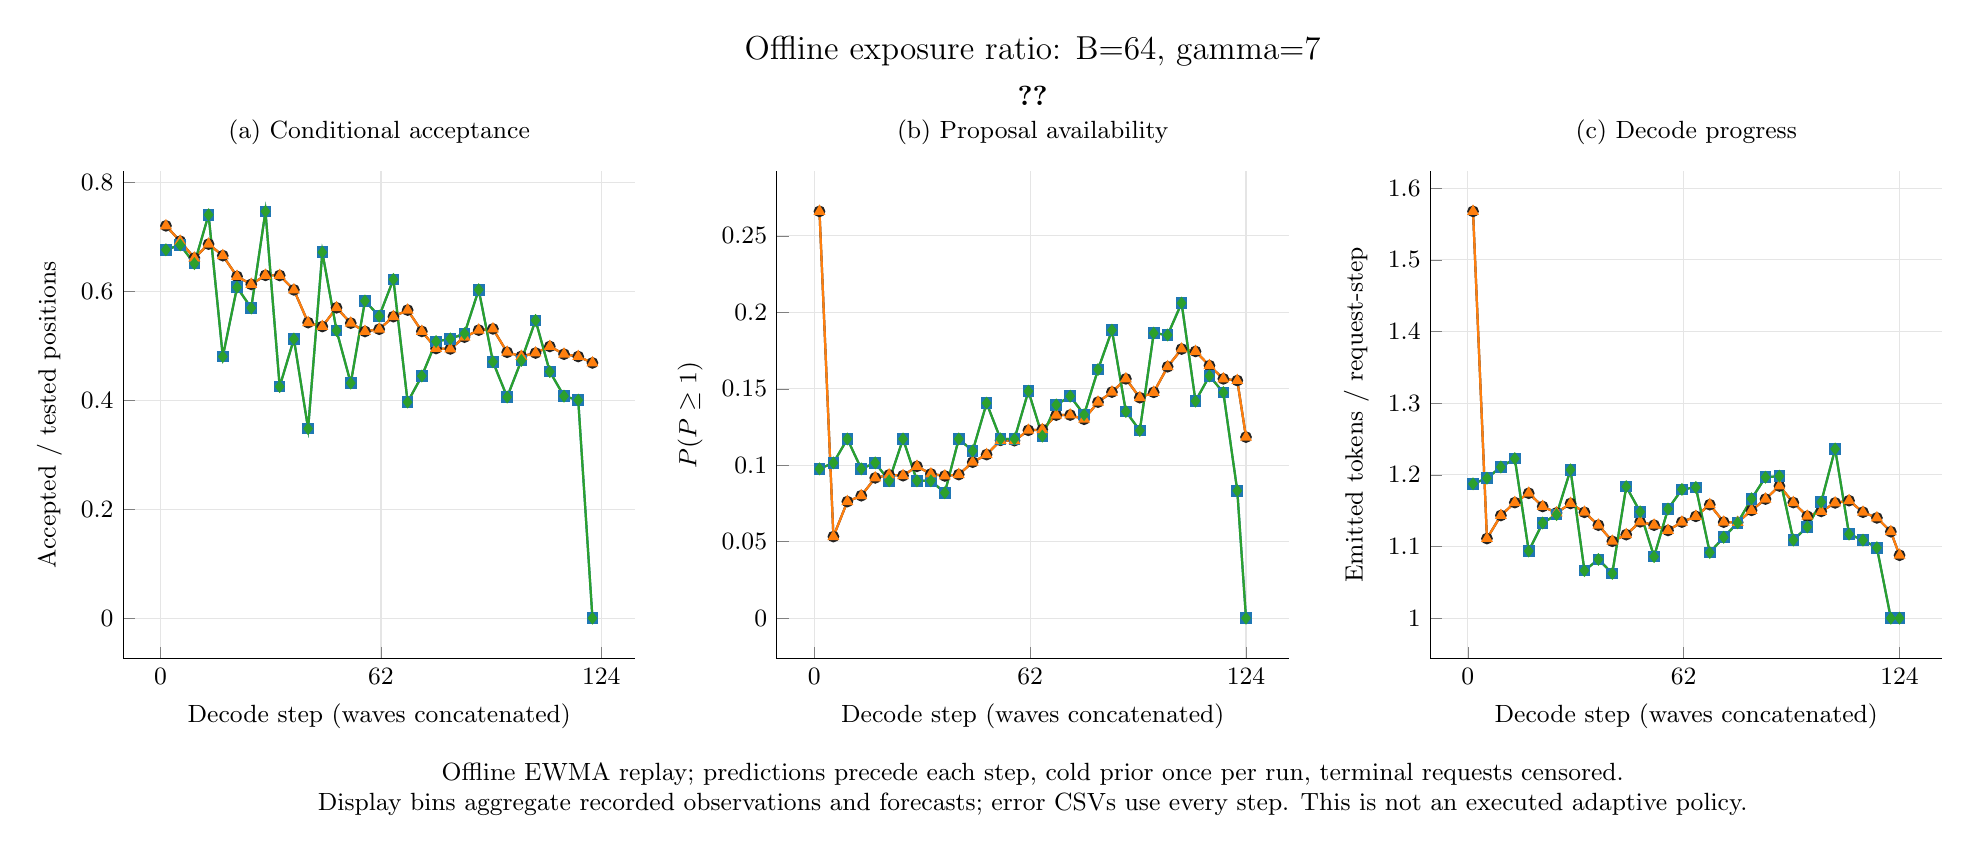
\begin{tikzpicture}
\definecolor{series0}{HTML}{222222}
\definecolor{series1}{HTML}{1f77b4}
\definecolor{series2}{HTML}{ff7f0e}
\definecolor{series3}{HTML}{2ca02c}
\definecolor{series4}{HTML}{d62728}
\definecolor{series5}{HTML}{9467bd}
\definecolor{series6}{HTML}{8c564b}
\definecolor{series7}{HTML}{e377c2}
\begin{groupplot}[group style={group size=3 by 1,horizontal sep=1.8cm},width=6.5cm,height=6.2cm,scale only axis,grid=major,grid style={gray!20},axis lines*=left,tick label style={font=\small},label style={font=\small},title style={font=\small},unbounded coords=jump]
\nextgroupplot[title={(a) Conditional acceptance},xlabel={Decode step (waves concatenated)},ylabel={Accepted / tested positions},xtick={0,62,124},xticklabels={0,62,124},scaled y ticks=false,yticklabel style={/pgf/number format/fixed,/pgf/number format/precision=2},legend columns=4,legend to name=sharedlegend,legend style={draw=none,font=\small,/tikz/every even column/.append style={column sep=8pt}}]
\addplot+[color=series0,mark=*,mark size=1.7pt,mark options={fill=series0,draw=series0},line width=0.8pt] coordinates {(1.5,0.719998662845) (5.5,0.691766983145) (9.5,0.660782017253) (13.5,0.686410579016) (17.5,0.665233156405) (21.5,0.627120855103) (25.5,0.612531144397) (29.5,0.629159353308) (33.5,0.628897678604) (37.5,0.602455883638) (41.5,0.542330453366) (45.5,0.53518433711) (49.5,0.569631075321) (53.5,0.541414987477) (57.5,0.526111986918) (61.5,0.530233393423) (65.5,0.553332770146) (69.5,0.565345571944) (73.5,0.526245217377) (77.5,0.494864476583) (81.5,0.494081888067) (85.5,0.515748519276) (89.5,0.528600932558) (93.5,0.530886416394) (97.5,0.48796485194) (101.5,0.480410115356) (105.5,0.486590686301) (109.5,0.498631277386) (113.5,0.484470957046) (117.5,0.480160633649) (121.5,0.468406180965) (124,nan)};
\addlegendentry{run 0: forecast}
\addplot+[only marks,forget plot,color=series0,mark=o,mark size=2.1pt,mark options={fill=white,line width=0.45pt}] coordinates {};
\addplot+[color=series1,mark=square*,mark size=1.7pt,mark options={fill=series1,draw=series1},line width=0.8pt] coordinates {(1.5,0.676056338028) (5.5,0.684931506849) (9.5,0.650602409639) (13.5,0.74025974026) (17.5,0.48) (21.5,0.607142857143) (25.5,0.569230769231) (29.5,0.746478873239) (33.5,0.425) (37.5,0.512195121951) (41.5,0.347826086957) (45.5,0.671428571429) (49.5,0.527777777778) (53.5,0.43137254902) (57.5,0.582089552239) (61.5,0.55421686747) (65.5,0.621621621622) (69.5,0.396551724138) (73.5,0.444444444444) (77.5,0.507692307692) (81.5,0.5125) (85.5,0.522222222222) (89.5,0.602739726027) (93.5,0.470588235294) (97.5,0.405797101449) (101.5,0.472972972973) (105.5,0.546511627907) (109.5,0.452380952381) (113.5,0.407407407407) (117.5,0.4) (121.5,0) (124,nan)};
\addlegendentry{run 0: observed}
\addplot+[only marks,forget plot,color=series1,mark=o,mark size=2.1pt,mark options={fill=white,line width=0.45pt}] coordinates {};
\addplot+[color=series2,mark=triangle*,mark size=1.7pt,mark options={fill=series2,draw=series2},line width=0.8pt] coordinates {(1.5,0.719998662845) (5.5,0.691766983145) (9.5,0.660782017253) (13.5,0.686410579016) (17.5,0.665233156405) (21.5,0.627120855103) (25.5,0.612531144397) (29.5,0.629159353308) (33.5,0.628897678604) (37.5,0.602455883638) (41.5,0.542330453366) (45.5,0.53518433711) (49.5,0.569631075321) (53.5,0.541414987477) (57.5,0.526111986918) (61.5,0.530233393423) (65.5,0.553332770146) (69.5,0.565345571944) (73.5,0.526245217377) (77.5,0.494864476583) (81.5,0.494081888067) (85.5,0.515748519276) (89.5,0.528600932558) (93.5,0.530886416394) (97.5,0.48796485194) (101.5,0.480410115356) (105.5,0.486590686301) (109.5,0.498631277386) (113.5,0.484470957046) (117.5,0.480160633649) (121.5,0.468406180965) (124,nan)};
\addlegendentry{run 1: forecast}
\addplot+[only marks,forget plot,color=series2,mark=o,mark size=2.1pt,mark options={fill=white,line width=0.45pt}] coordinates {};
\addplot+[color=series3,mark=diamond*,mark size=1.7pt,mark options={fill=series3,draw=series3},line width=0.8pt] coordinates {(1.5,0.676056338028) (5.5,0.684931506849) (9.5,0.650602409639) (13.5,0.74025974026) (17.5,0.48) (21.5,0.607142857143) (25.5,0.569230769231) (29.5,0.746478873239) (33.5,0.425) (37.5,0.512195121951) (41.5,0.347826086957) (45.5,0.671428571429) (49.5,0.527777777778) (53.5,0.43137254902) (57.5,0.582089552239) (61.5,0.55421686747) (65.5,0.621621621622) (69.5,0.396551724138) (73.5,0.444444444444) (77.5,0.507692307692) (81.5,0.5125) (85.5,0.522222222222) (89.5,0.602739726027) (93.5,0.470588235294) (97.5,0.405797101449) (101.5,0.472972972973) (105.5,0.546511627907) (109.5,0.452380952381) (113.5,0.407407407407) (117.5,0.4) (121.5,0) (124,nan)};
\addlegendentry{run 1: observed}
\addplot+[only marks,forget plot,color=series3,mark=o,mark size=2.1pt,mark options={fill=white,line width=0.45pt}] coordinates {};
\nextgroupplot[title={(b) Proposal availability},xlabel={Decode step (waves concatenated)},ylabel={$P(P \geq 1)$},xtick={0,62,124},xticklabels={0,62,124},scaled y ticks=false,yticklabel style={/pgf/number format/fixed,/pgf/number format/precision=2}]
\addplot+[color=series0,mark=*,mark size=1.7pt,mark options={fill=series0,draw=series0},line width=0.8pt] coordinates {(1.5,0.266015625) (5.5,0.0533539453125) (9.5,0.0762453672695) (13.5,0.0800948979655) (17.5,0.0917397156802) (21.5,0.0937076149578) (25.5,0.0931952380488) (29.5,0.0992938331838) (33.5,0.0943134808269) (37.5,0.0930185278955) (41.5,0.0939001592773) (45.5,0.102021957002) (49.5,0.106984262239) (53.5,0.116307218205) (57.5,0.116106040864) (61.5,0.122868579661) (65.5,0.123284561227) (69.5,0.132787295292) (73.5,0.132845515946) (77.5,0.130076878496) (81.5,0.141285005056) (85.5,0.147842216117) (89.5,0.156503407865) (93.5,0.144188724587) (97.5,0.147703585838) (101.5,0.164420375744) (105.5,0.175998026122) (109.5,0.174432194797) (113.5,0.165158500318) (117.5,0.156499184548) (121.5,0.1554080804) (124,0.118408886529)};
\addplot+[only marks,forget plot,color=series0,mark=o,mark size=2.1pt,mark options={fill=white,line width=0.45pt}] coordinates {};
\addplot+[color=series1,mark=square*,mark size=1.7pt,mark options={fill=series1,draw=series1},line width=0.8pt] coordinates {(1.5,0.09765625) (5.5,0.1015625) (9.5,0.1171875) (13.5,0.09765625) (17.5,0.1015625) (21.5,0.08984375) (25.5,0.1171875) (29.5,0.08984375) (33.5,0.08984375) (37.5,0.08203125) (41.5,0.1171875) (45.5,0.109375) (49.5,0.140625) (53.5,0.1171875) (57.5,0.1171875) (61.5,0.1484375) (65.5,0.119047619048) (69.5,0.139442231076) (73.5,0.145161290323) (77.5,0.133064516129) (81.5,0.162601626016) (85.5,0.188284518828) (89.5,0.135135135135) (93.5,0.122727272727) (97.5,0.186363636364) (101.5,0.185185185185) (105.5,0.206030150754) (109.5,0.141975308642) (113.5,0.158415841584) (117.5,0.147540983607) (121.5,0.0833333333333) (124,0)};
\addplot+[only marks,forget plot,color=series1,mark=o,mark size=2.1pt,mark options={fill=white,line width=0.45pt}] coordinates {};
\addplot+[color=series2,mark=triangle*,mark size=1.7pt,mark options={fill=series2,draw=series2},line width=0.8pt] coordinates {(1.5,0.266015625) (5.5,0.0533539453125) (9.5,0.0762453672695) (13.5,0.0800948979655) (17.5,0.0917397156802) (21.5,0.0937076149578) (25.5,0.0931952380488) (29.5,0.0992938331838) (33.5,0.0943134808269) (37.5,0.0930185278955) (41.5,0.0939001592773) (45.5,0.102021957002) (49.5,0.106984262239) (53.5,0.116307218205) (57.5,0.116106040864) (61.5,0.122868579661) (65.5,0.123284561227) (69.5,0.132787295292) (73.5,0.132845515946) (77.5,0.130076878496) (81.5,0.141285005056) (85.5,0.147842216117) (89.5,0.156503407865) (93.5,0.144188724587) (97.5,0.147703585838) (101.5,0.164420375744) (105.5,0.175998026122) (109.5,0.174432194797) (113.5,0.165158500318) (117.5,0.156499184548) (121.5,0.1554080804) (124,0.118408886529)};
\addplot+[only marks,forget plot,color=series2,mark=o,mark size=2.1pt,mark options={fill=white,line width=0.45pt}] coordinates {};
\addplot+[color=series3,mark=diamond*,mark size=1.7pt,mark options={fill=series3,draw=series3},line width=0.8pt] coordinates {(1.5,0.09765625) (5.5,0.1015625) (9.5,0.1171875) (13.5,0.09765625) (17.5,0.1015625) (21.5,0.08984375) (25.5,0.1171875) (29.5,0.08984375) (33.5,0.08984375) (37.5,0.08203125) (41.5,0.1171875) (45.5,0.109375) (49.5,0.140625) (53.5,0.1171875) (57.5,0.1171875) (61.5,0.1484375) (65.5,0.119047619048) (69.5,0.139442231076) (73.5,0.145161290323) (77.5,0.133064516129) (81.5,0.162601626016) (85.5,0.188284518828) (89.5,0.135135135135) (93.5,0.122727272727) (97.5,0.186363636364) (101.5,0.185185185185) (105.5,0.206030150754) (109.5,0.141975308642) (113.5,0.158415841584) (117.5,0.147540983607) (121.5,0.0833333333333) (124,0)};
\addplot+[only marks,forget plot,color=series3,mark=o,mark size=2.1pt,mark options={fill=white,line width=0.45pt}] coordinates {};
\nextgroupplot[title={(c) Decode progress},xlabel={Decode step (waves concatenated)},ylabel={Emitted tokens / request-step},xtick={0,62,124},xticklabels={0,62,124},scaled y ticks=false,yticklabel style={/pgf/number format/fixed,/pgf/number format/precision=2}]
\addplot+[color=series0,mark=*,mark size=1.7pt,mark options={fill=series0,draw=series0},line width=0.8pt] coordinates {(1.5,1.56768323309) (5.5,1.11113879436) (9.5,1.14334963872) (13.5,1.161337981) (17.5,1.17438132198) (21.5,1.15587759109) (25.5,1.14696460867) (29.5,1.16010723384) (33.5,1.14777310936) (37.5,1.12980160639) (41.5,1.10734675683) (45.5,1.11660732535) (49.5,1.13449799251) (53.5,1.12984057034) (57.5,1.1224396636) (61.5,1.1341172854) (65.5,1.14215106669) (69.5,1.15842099647) (73.5,1.13405367656) (77.5,1.13373080567) (81.5,1.15051854428) (85.5,1.16624700635) (89.5,1.18442348375) (93.5,1.16135858447) (97.5,1.14228021663) (101.5,1.14903701146) (105.5,1.16090875226) (109.5,1.16403735605) (113.5,1.14793218616) (117.5,1.13996680142) (121.5,1.12070083402) (124,1.08782468842)};
\addplot+[only marks,forget plot,color=series0,mark=o,mark size=2.1pt,mark options={fill=white,line width=0.45pt}] coordinates {};
\addplot+[color=series1,mark=square*,mark size=1.7pt,mark options={fill=series1,draw=series1},line width=0.8pt] coordinates {(1.5,1.1875) (5.5,1.1953125) (9.5,1.2109375) (13.5,1.22265625) (17.5,1.09375) (21.5,1.1328125) (25.5,1.14453125) (29.5,1.20703125) (33.5,1.06640625) (37.5,1.08203125) (41.5,1.0625) (45.5,1.18359375) (49.5,1.1484375) (53.5,1.0859375) (57.5,1.15234375) (61.5,1.1796875) (65.5,1.18253968254) (69.5,1.09163346614) (73.5,1.11290322581) (77.5,1.13306451613) (81.5,1.16666666667) (85.5,1.19665271967) (89.5,1.1981981982) (93.5,1.10909090909) (97.5,1.12727272727) (101.5,1.16203703704) (105.5,1.23618090452) (109.5,1.11728395062) (113.5,1.10891089109) (117.5,1.09836065574) (121.5,1) (124,1)};
\addplot+[only marks,forget plot,color=series1,mark=o,mark size=2.1pt,mark options={fill=white,line width=0.45pt}] coordinates {};
\addplot+[color=series2,mark=triangle*,mark size=1.7pt,mark options={fill=series2,draw=series2},line width=0.8pt] coordinates {(1.5,1.56768323309) (5.5,1.11113879436) (9.5,1.14334963872) (13.5,1.161337981) (17.5,1.17438132198) (21.5,1.15587759109) (25.5,1.14696460867) (29.5,1.16010723384) (33.5,1.14777310936) (37.5,1.12980160639) (41.5,1.10734675683) (45.5,1.11660732535) (49.5,1.13449799251) (53.5,1.12984057034) (57.5,1.1224396636) (61.5,1.1341172854) (65.5,1.14215106669) (69.5,1.15842099647) (73.5,1.13405367656) (77.5,1.13373080567) (81.5,1.15051854428) (85.5,1.16624700635) (89.5,1.18442348375) (93.5,1.16135858447) (97.5,1.14228021663) (101.5,1.14903701146) (105.5,1.16090875226) (109.5,1.16403735605) (113.5,1.14793218616) (117.5,1.13996680142) (121.5,1.12070083402) (124,1.08782468842)};
\addplot+[only marks,forget plot,color=series2,mark=o,mark size=2.1pt,mark options={fill=white,line width=0.45pt}] coordinates {};
\addplot+[color=series3,mark=diamond*,mark size=1.7pt,mark options={fill=series3,draw=series3},line width=0.8pt] coordinates {(1.5,1.1875) (5.5,1.1953125) (9.5,1.2109375) (13.5,1.22265625) (17.5,1.09375) (21.5,1.1328125) (25.5,1.14453125) (29.5,1.20703125) (33.5,1.06640625) (37.5,1.08203125) (41.5,1.0625) (45.5,1.18359375) (49.5,1.1484375) (53.5,1.0859375) (57.5,1.15234375) (61.5,1.1796875) (65.5,1.18253968254) (69.5,1.09163346614) (73.5,1.11290322581) (77.5,1.13306451613) (81.5,1.16666666667) (85.5,1.19665271967) (89.5,1.1981981982) (93.5,1.10909090909) (97.5,1.12727272727) (101.5,1.16203703704) (105.5,1.23618090452) (109.5,1.11728395062) (113.5,1.10891089109) (117.5,1.09836065574) (121.5,1) (124,1)};
\addplot+[only marks,forget plot,color=series3,mark=o,mark size=2.1pt,mark options={fill=white,line width=0.45pt}] coordinates {};
\end{groupplot}
\path (group c1r1.north west) -- node[above=1.2cm,font=\large] {Offline exposure ratio: B=64, gamma=7} (group c3r1.north east);
\path (group c1r1.north west) -- node[above=0.7cm] {\ref{sharedlegend}} (group c3r1.north east);
\path (group c1r1.south west) -- node[below=1.2cm,align=center,font=\small] {Offline EWMA replay; predictions precede each step, cold prior once per run, terminal requests censored.\\Display bins aggregate recorded observations and forecasts; error CSVs use every step. This is not an executed adaptive policy.} (group c3r1.south east);
\end{tikzpicture}
\end{document}
